The output of the development phase is an artifact which is a \gls{VSCode} extension.
The artifact is a \texttt{.vsix} file, and can be installed in a \gls{Gitpod} workspace.
The following results are from \gls{Gitpod} using \gls{VSCode} as the editor frontend, not \gls{Theia}\footnote{VSCode is the default for Gitpod, instead of Theia~\cite{georgetsiolisMenuEntryGitpod2019,svenefftingeProductRoadmapQ1}.}.
One way to install it\footnote{The ``best'' way is to publish the extension to OpenVSX, and search for it in the extensions panel.}, is to upload the \texttt{.vsix} file to the workspace, right clicking on it and selecting ``Install Extension VSIX''.
When installed in the \acrshort{IDE}, it is shown in the extensions panel as \textit{Ecore Tree-editor}, shown in \cref{fig:gitpod-ext-installed}.

\begin{figure}[H]  % order of priority: h here, t top, b bottom, p page
  \centering
  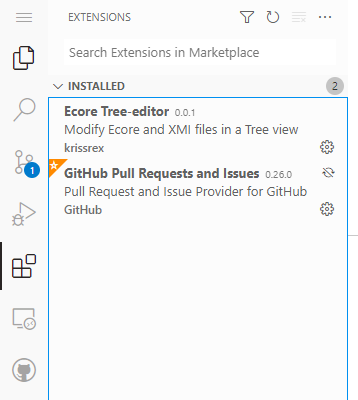
\includegraphics[width=0.6\textwidth]{figures/gitpod-vscode-extensions-installed.png}
  \caption[Tree Editor Extension installed in Gitpod]{The extension is installed as \textit{Ecore Tree-editor} in Gitpod with VSCode.}\label{fig:gitpod-ext-installed}
\end{figure}

\subsection{Custom Editor}

This extension adds a new Custom Editor, which is automatically opened when the user opens a \texttt{.ecore}, \texttt{.genmodel} or \texttt{.xmi} file.
The model file is loaded and transformed by the extension, and presented as a tree to the user.

\begin{figure}[H]  % order of priority: h here, t top, b bottom, p page
  \centering
  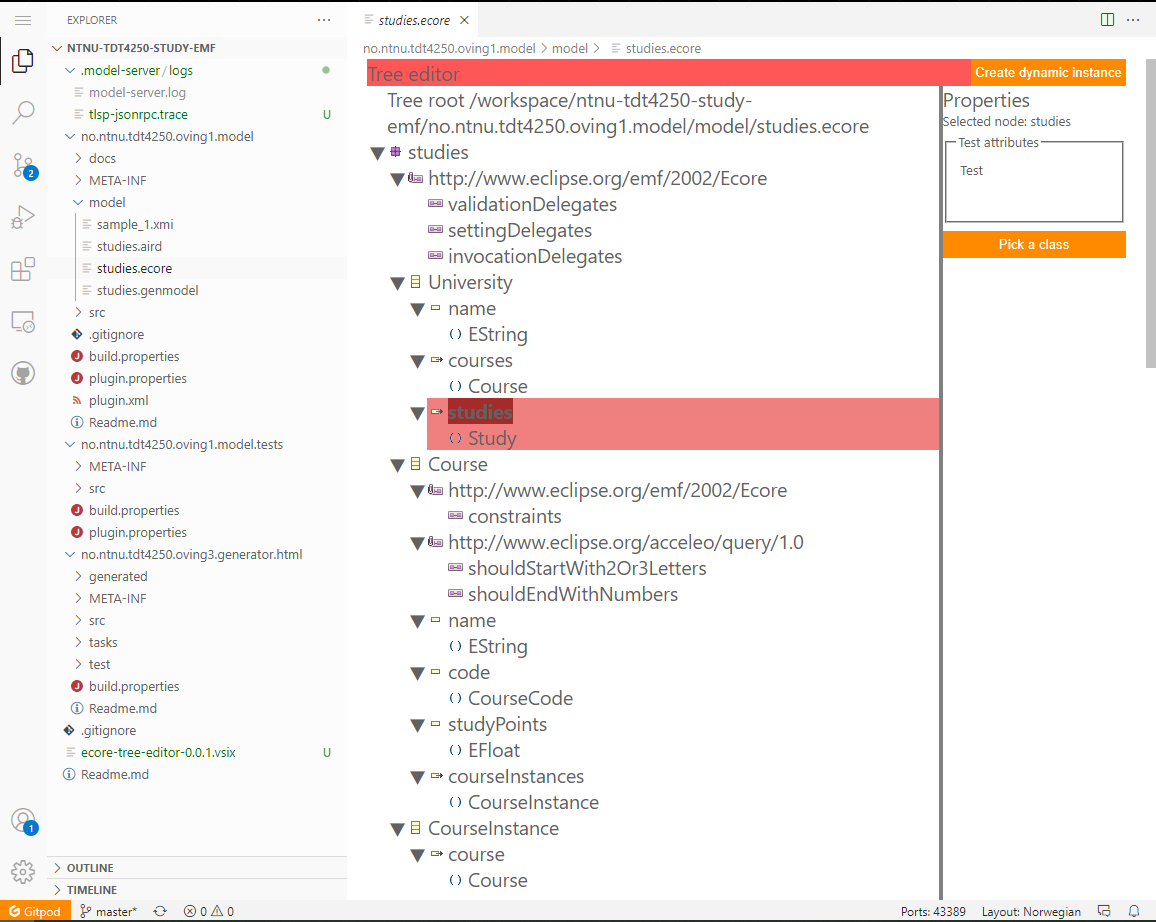
\includegraphics[width=\textwidth]{figures/gitpod-vscode-ecore-editor-studyemf.png}
  \caption[Tree Editor Extension showing studies.ecore]{The Tree Editor Extension has opened a Custom Editor for the \texttt{studies.ecore} file.}\label{fig:gitpod-ext-tree-ecore}
\end{figure}

\paragraph{Example model}
An \gls{Ecore} model made in \gls{TDT4250} in 2019 has been used as an example to demonstrate the artifact.
The \texttt{.ecore} file is opened in \cref{fig:gitpod-ext-tree-ecore}.
This figure shows three columns, from left to right: the default \gls{VSCode} file explorer, the custom editor's master layout (tree structure), and the custom editor's detail layout (properties sheet).

\paragraph{Action bar}
There is also a red action bar at the top, with an orange action button to create a new dynamic instance.
The action buttons shown will vary, depending on what the selected node is.
The orange color of the button is coming from the color theme of the \gls{VSCode} editor.
With a dark theme, this action button could be blue, for example.

\paragraph{Master layout}
The master layout can show multiple roots.
In this document,  single root is shown for the ``studies.ecore'' file.
The root node is a ``studies'' package, with children displayed below.
This node has a label, ``studies'', and a specific icon indicating it is a package --- the purple box with a cross.
The icons used are the same ones used in \gls{Eclipse} for the Sample Reflective Ecore Editor (see \cref{sec:sample-reflective-editor}), and depend on the type of node.

Clicking the black triangle next to a node will collapse it, hiding its children and rotating the triangle 90 degrees counter-clockwise.

Inside the master layout, a node is selected in dark red, with the label ``studies''.
Its child node ``Study'' is also highlighted, in a lighter red.
(Note that the colors of selected nodes were arbitrarily chosen during development, and could be changed to give more contrast with the node's label.)
A node can be selected by clicking on it, and holding \texttt{ctrl} will add to the selection, allowing multiple nodes to be selected.

Dragging a node in the hierarchy and dropping it on a node, should change this node's parent.
Right clicking a node will open a context menu, with the possible children nodes to add.
Dropping a node on an invalid parent will be prevented, by using a hierarchy schema, and indicated by changing the mouse cursor to a ``forbidden'' icon\footnote{Note that drag-and-drop and node creation are not currently implemented, only accounted for by the design, by using a hierarchy schema.}.


\paragraph{Detail layout}
The detail layout has a property sheet, currently showing a unfinished example form.
This layout should use the \textit{JSON-Forms} library to render properties, based on the node's properties and a \textit{UI schema} for that node type.


\subsection{IDE Commands}

The extension also provides Commands to \gls{VSCode}.
These are actions that can be invoked at any time.
The student can invoke them from the Command Palette\footnote{Press \texttt{F1}, or \texttt{ctrl + shift + P} (command on mac), or \texttt{Menu $\rightarrow$ View $\rightarrow$ Command palette}} by typing ``Ecore'' or another part of the command's name.
A screenshot is shown in \cref{fig:gitpod-ext-newmodel}, with a command to create a new model file.
This file will have the minimum \acrshort{XMI} contents required for a blank model.

\begin{figure}[H]  % order of priority: h here, t top, b bottom, p page
  \centering
  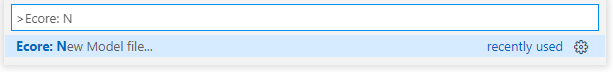
\includegraphics[width=\textwidth]{figures/gitpod-vscode-newmodel.png}
  \caption[Tree Editor Extension Custom Commands]{The Tree Editor Extension adds custom commands to the Command Palette. One of them is shown here, named \textit{Ecore: New Model file\ldots}.}\label{fig:gitpod-ext-newmodel}
\end{figure}

\subsection{Genmodel and Model Instance}

The editor can open a \texttt{.genmodel} file or a \texttt{.xmi} model instance file as well.
The GenModel is shown in \cref{fig:gitpod-ext-genmodel}, and the dynamic instance in \cref{fig:gitpod-ext-dynamic}.
This will show two roots in the editor, as the original \texttt{.ecore} model is related to the opened file.
One root is the GenModel or model instance, and the other root is the study model.

The GenModel editor is not specialized, so it renders the tree as any other \gls{Ecore} model.

\begin{figure}[H]  % order of priority: h here, t top, b bottom, p page
  \centering
  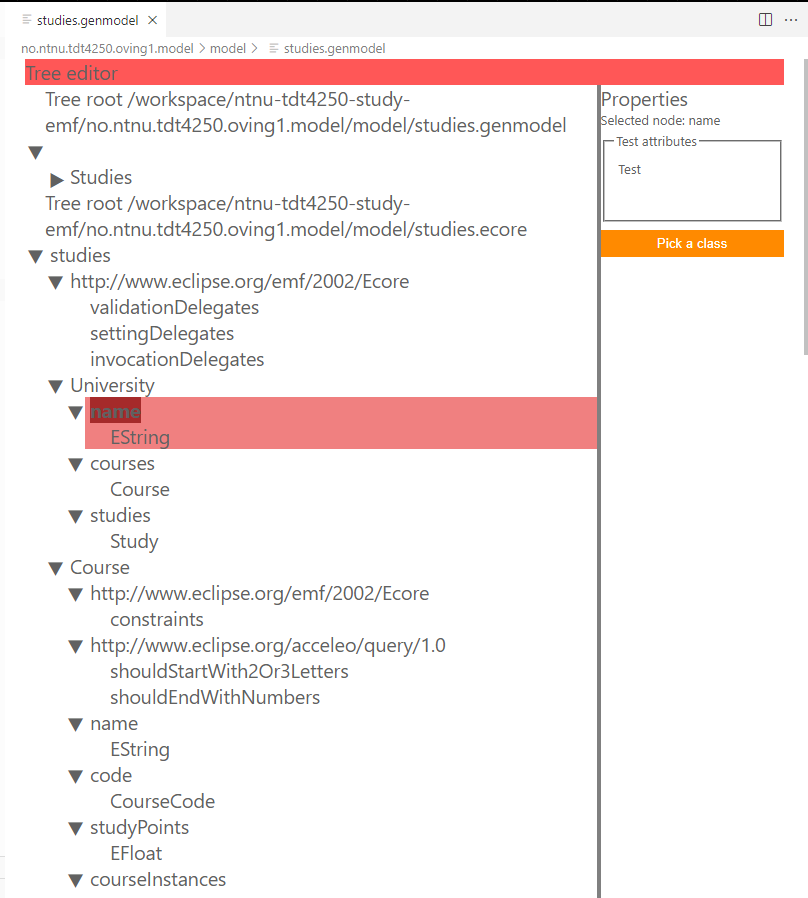
\includegraphics[width=\textwidth]{figures/gitpod-vscode-genmodel.png}
  \caption[Tree Editor Extension showing studies.genmodel]{The Tree Editor Extension with the \texttt{studies.genmodel} file open. It has two roots, the GenModel and the model. The GenModel is collapsed/hidden at the ``Studies'' node.}\label{fig:gitpod-ext-genmodel}
\end{figure}

\begin{figure}[H]  % order of priority: h here, t top, b bottom, p page
  \centering
  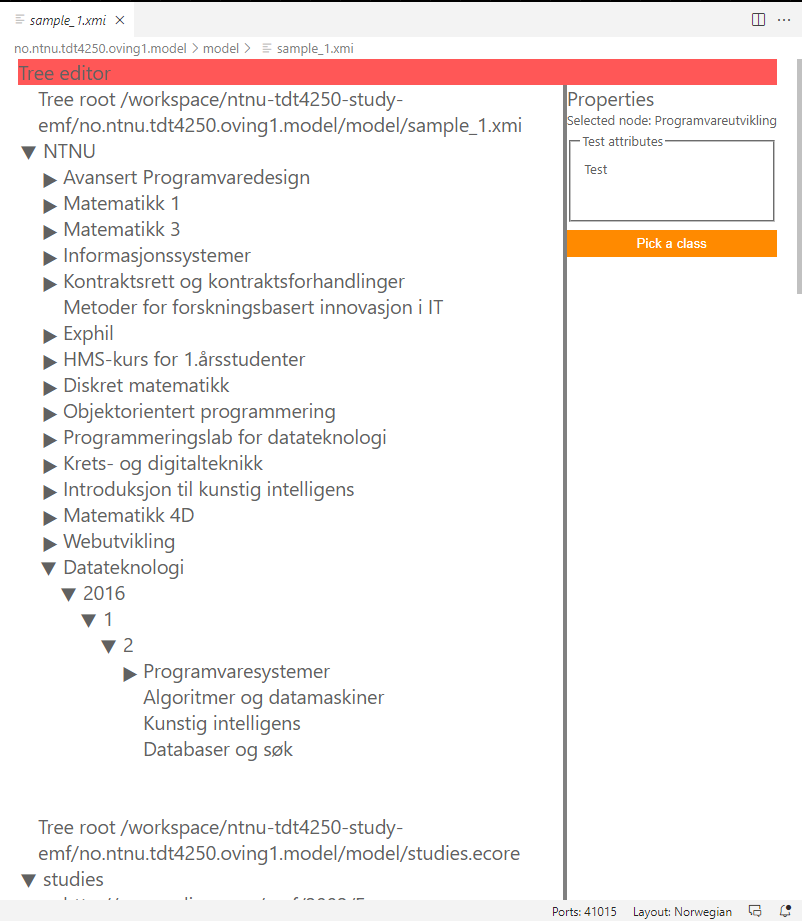
\includegraphics[width=\textwidth]{figures/gitpod-vscode-xmi-study-instance.png}
  \caption[Tree Editor Extension showing a dynamic instance]{The Tree Editor Extension with the \texttt{sample\_1.xmi} dynamic instance open. This is data that conforms to the model defined in \texttt{studies.ecore}.}\label{fig:gitpod-ext-dynamic}
\end{figure}


\subsection{Configuration and Logging}

The extension has configuration options that a user can set.
One such option is the logging level, a threshold to hide log messages in the log panel.
The extension can also log internal events and messages to a Output panel in \gls{VSCode}, for the user to debug and identify errors.
The configuration and output panel are shown in \cref{fig:gitpod-ext-config-log}.

\begin{figure}[htbp]  % order of priority: h here, t top, b bottom, p page
  \centering
  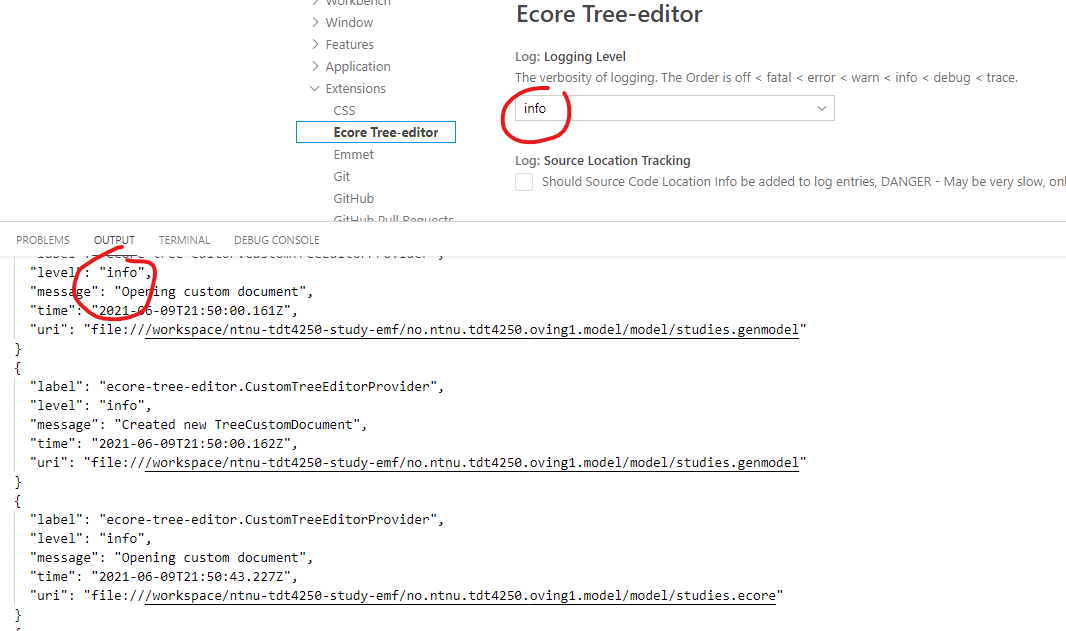
\includegraphics[width=\textwidth]{figures/gitpod-vscode-config-and-logging.png}
  \caption[Tree Editor Extension with configuration and logging]{The Tree Editor Extension adds configuration options to the \gls{VSCode} settings menu, shown in the top right.
  The extension also adds log outputs to a Output panel.
  The figure is annotated with two red circles.
  The upper circle is indicating the configuration option to filter the output based on log level.
  The lower circle is highlighting that same log level from a message in the output panel.}\label{fig:gitpod-ext-config-log}
\end{figure}


\iffalse{
% * Steps:
% 1. Sign up to Gitpod.io with GitHub user
% 2. Go to Settings. Set default IDE as VSCode. (It will be the default soon % % https://github.com/gitpod-io/gitpod/issues/3989#issuecomment-822246441)
% 3. Open %https://gitpod.io/#https://github.com/krissrex/ntnu-tdt4250-study-emf % to get a Workspace in gitpod with an EMF project. The Tree Language Server does % not support multi-workspace.
% 4. Build the extension locally to obtain a .vsix file (or download a build from % somewhere)
% 5. Upload the .vsix to the project workspace by drag-and-drop.
% 6. Right-click the .vsix file in VSCode/Gitpod, select "Install Extension VSIX".
% 7. Wait for "Completed installing Ecore Tree-editor extension from VSIX" popup % in bottom right corner.
% 8. Open folder with models: "no.ntnu.tdt4250.oving1.model/model"
% 9. Click model file: "studies.ecore"
% 10. Click genmodel file: "studies.genmodel"
% 11. Click dynamic instance file: "sample_1.xmi"
}
\fi

\FloatBarrier % Prevent figures running into the next section